\documentclass[12pt]{article}
\usepackage{amsmath,amssymb,mathtools}
\usepackage{tikz}

\begin{document}

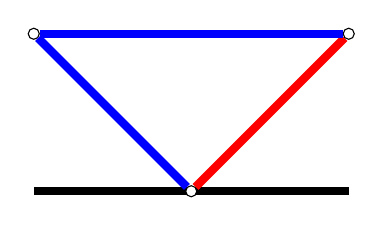
\begin{tikzpicture}
\tikzstyle{hackennode}=[draw,circle,inner sep=0,minimum size=4pt]
\tikzstyle{hackenline}=[line width=3pt]
    \draw[hackenline,black] (0,0) -- (4,0);
    \node[hackennode][fill= white] (1) at (2,0) {}; 
    \node[hackennode][fill= white] (2) at (0,2) {}; 
    \node[hackennode][fill= white] (3) at (4,2) {};

    \draw[hackenline,blue] (1) -- (2);
    \draw[hackenline,red] (1) -- (3);
    \draw[hackenline,blue] (2) -- (3);
\end{tikzpicture}

\end{document}